\begin{ZhChapter}

\chapter{BLE Mesh拓樸建立機制設計}

\section{問題分析}

\subsection{BLE Mesh拓樸建立問題}

在原生FruityMesh架構中,節點的建立與連線並未針對資料匯集或匯出端進行特別設計,因此整體網路並無明確的Root節點。其封包傳輸方式主要採用廣播機制,即每當節點產生封包時,會向所有相鄰節點廣播傳送,期望藉由鄰近節點的重傳將封包推進至目的地。雖然此方法具備一定的自我修復能力,但在多節點、大範圍的Mesh網路中,極易導致封包重複傳送與碰撞,進而產生所謂的「廣播風暴」現象,嚴重影響整體網路效能與穩定性。

為了解決此問題,研究中引入DOT(Destination Oriented Transmission)機制\cite{112TIT00392032},將原先的無向廣播傳輸改為目的導向的封包路由方式,透過樹狀拓樸的建立使資料傳輸路徑更具方向性與效率性。然而,導入DOT排程機制的前提之一,是整個BLE Mesh網路需具備清楚的階層結構,而Sink節點(資料匯集端)必須作為整體樹狀拓樸的根節點。唯有如此,封包才能沿著既定的父子節點路徑,自節點有效匯流至Sink節點,達成DOT排程所需的單向、無冗餘傳輸目標。

然而,由於FruityMesh原生設計並非以Sink節點為中心的拓樸為出發點,現有拓樸建立流程尚無法保證Sink節點必然成為根節點。在未進行拓樸控制調整的情況下,可能出現Sink位置偏移、處於樹葉節點甚至中繼節點等非理想情境。因此,若要在FruityMesh架構中有效實作DOT排程機制,勢必需重新設計拓樸建立邏輯,強制指定使Sink節點始終位於拓樸樹的根部,即使在斷線並重新連線的情況下,亦能恢復其根節點角色,確保網路穩定性與傳輸效能。

\subsection{BLE Mesh封包傳輸問題}

在基於FruityMesh的藍牙低功耗網狀網路(BLE Mesh)傳輸機制設計中,\cite{112TIT00392032}研究已針對封包延遲與封包抵達率等品質指標進行優化,並取得初步成效。該研究藉由導入DOT與DOST排程機制,成功改善了大部分的傳輸延遲與資料完整性。然而,即使在優化機制下,網路中仍不時出現封包遺失(掉封包)與重傳現象,顯示目前的傳輸機制尚存在進一步提升的空間。

造成封包掉落與重傳的關鍵因素之一,在於BLE Mesh網路的流量集中特性。由於整體網路皆以Sink節點作為封包的最終目的地,所有資料封包最終皆會匯集至該節點,導致越接近Sink的節點需承擔更多的中繼與轉發任務。這種負載不均的現象將使中樞節點在短時間內接收到大量傳輸要求,導致中樞節點的Sent buffer資源迅速耗盡。一旦緩衝區爆滿,不僅無法即時處理新進封包,還可能造成排程延遲、封包掉落,進而引發重傳機制啟動,進一步加重網路負載。

為有效緩解此類壅塞現象,需從連線參數層級進行調整,特別是針對Connection Event(CE)與Connection Interval(CI)進行優化配置。透過適當調整CI間隔,可有效控制節點可傳輸封包的節奏與頻寬分配,進一步降低高負載節點的壓力,提升整體封包處理效率。結合連線參數調整機制,可以有效改善封包壅塞問題,以提升BLE Mesh網路在多節點、高流量情境下的服務品質(QoS)。

\section{BLE Mesh拓樸建立機制設計}

本論文提出改善FruityMesh的拓樸建立機制,確保Sink節點始終位於整體網路的根節點,並在斷線後能夠自動恢復其角色。此設計為後續的DOT排程機制提供穩定的基礎,如圖\ref{fig: 提出的拓樸建立流程圖}。

\begin{figure*}[htbp]
    \centering
    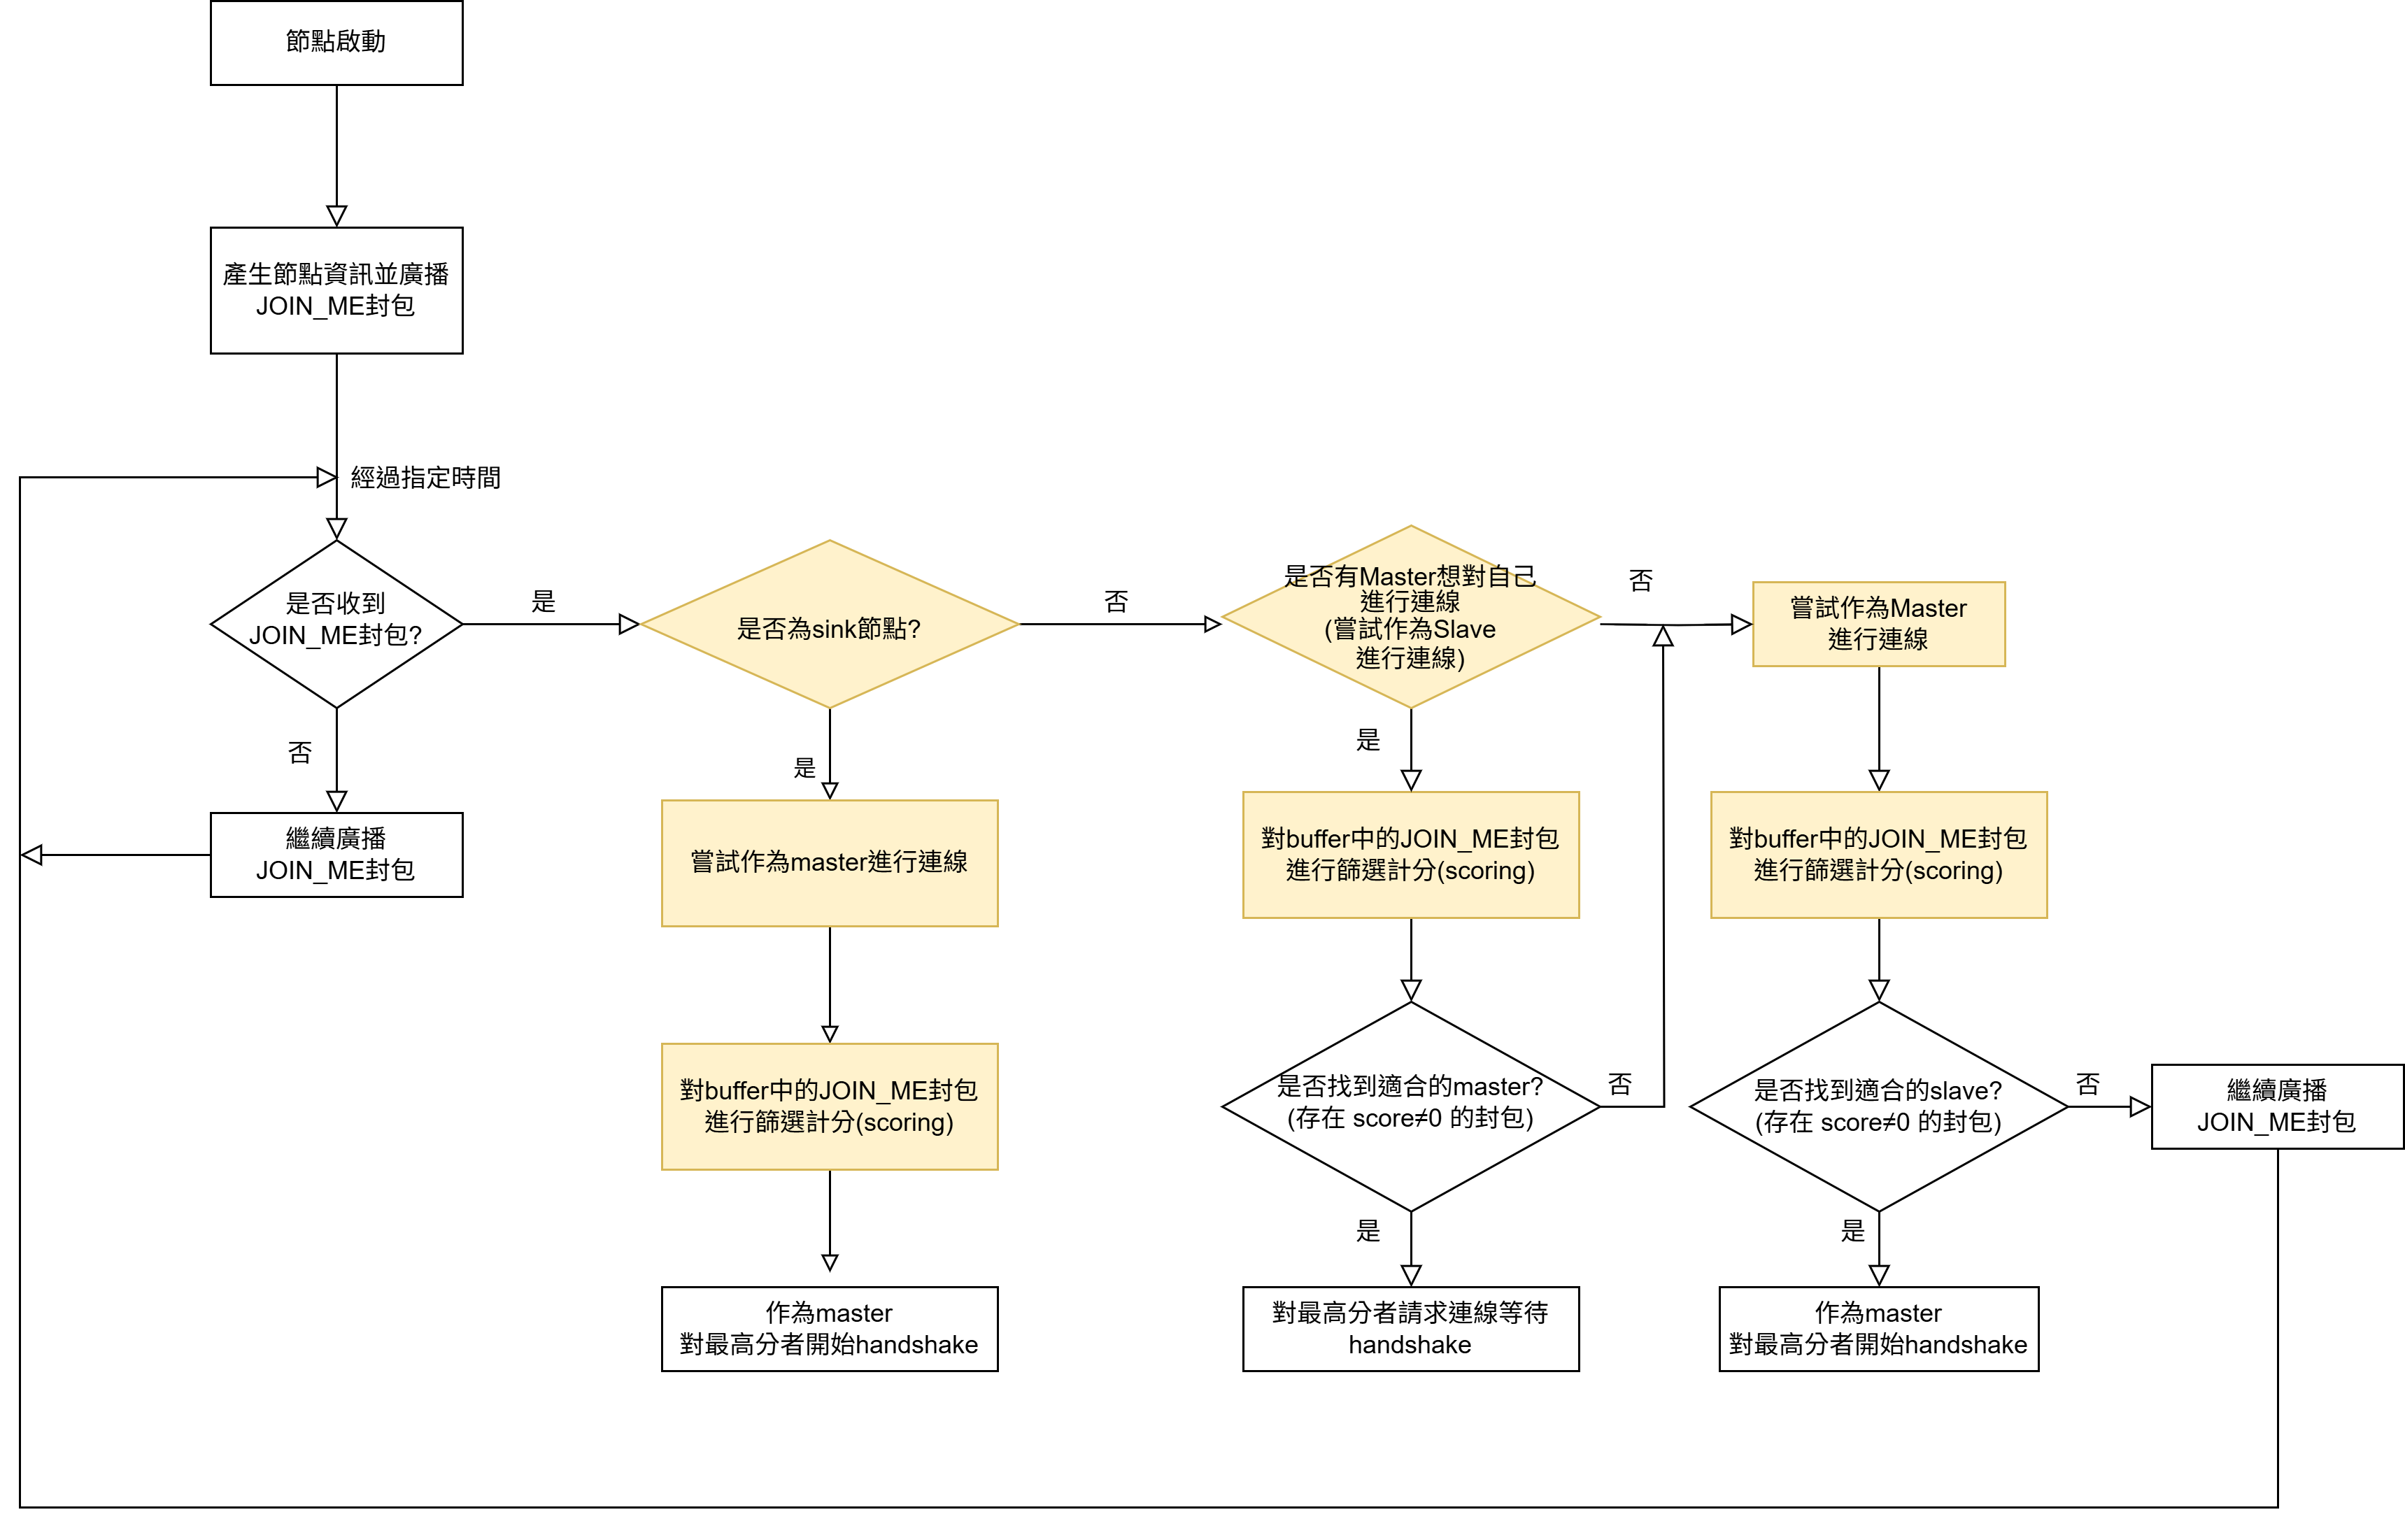
\includegraphics[width = 1\textwidth]{image/build-up_pro2.png}
    \caption{提出的拓樸建立流程圖}
    \label{fig: 提出的拓樸建立流程圖}
\end{figure*}

拓樸建立流程啟動時,每個節點在開機後會廣播包含自身節點資訊的JOIN\_ME封包。節點收到其他節點廣播的JOIN\_ME封包後,將其儲存於緩衝區中,並根據封包內容進行評分(scoring),以評估對方作為連線對象的適合程度。評分機制可依據鄰近程度、角色可用性(Master/Slave)、RSSI訊號強度或是否為Sink節點等條件進行加權計算。

若節點本身為指定的Sink節點,則會主動嘗試作為Master發起連線,以確保拓樸的根節點地位。同時,其他非Sink節點則會根據收到的JOIN\_ME封包內容與本地評分結果,決定是否以Slave或Master身分進行連線。

透過此機制設計,即使在節點斷線後重新加入網路時,也能根據評分與角色邏輯,回復正確的節點位置與角色,確保整體BLE Mesh網路拓樸的一致性與資料流的穩定性。

\subsection{決定最好的群組加入}

\begin{algorithm}
\caption{DetermineBestClusterAvailable Function}
\label{alg: DetermineBestClusterAvailable}
\begin{algorithmic}[1]
\State Initialize \texttt{result} as \texttt{NO\_NODES\_FOUND}
\State Get device type and assign to \texttt{deviceType}

\If{deviceType is \texttt{SINK} and outbound connections are available}
    \State \texttt{bestClusterAsMaster} $\gets$ \texttt{DetermineBestClusterAsMaster()}
    \If{\texttt{bestClusterAsMaster} $\neq$ null}
        \State Adjust \texttt{connectionIv} based on peer’s device type
        \State Attempt to connect as Master
        \If{connection succeeds}
            \State Update connection attempt time and count
        \EndIf
        \State Set \texttt{result.result} $\gets$ \texttt{CONNECT\_AS\_MASTER}
        \State Set \texttt{result.preferredPartner} $\gets$ bestClusterAsMaster.sender
        \State \Return result
    \EndIf
\Else
    \State Reset \texttt{currentAckId} to 0
    \State \texttt{bestClusterAsSlave} $\gets$ \texttt{DetermineBestClusterAsSlave()}

    \If{deviceType is \texttt{SINK}}
        \State \texttt{bestClusterAsSlave} $\gets$ null
    \EndIf

    \If{\texttt{bestClusterAsSlave} $\neq$ null}
        \State \texttt{currentAckId} $\gets$ bestClusterAsSlave.clusterId
        \If{\texttt{meshMaxInConnections == 1}}
            \State Check if any fresh connection exists (handshake not expired)
            \If{no fresh connection and \texttt{freeMeshInConnections == 0}}
                \If{clusterSize $\neq$ bestClusterAsSlave.clusterSize OR random trigger passed}
                    \State Force disconnect other mesh connections
                    \State Reset cluster size to 1
                    \State Generate new \texttt{clusterId}
                \EndIf
            \EndIf
        \EndIf
        \State Update JoinMe packet
        \State Set \texttt{result.result} $\gets$ \texttt{CONNECT\_AS\_SLAVE}
        \State Set \texttt{result.preferredPartner} $\gets$ bestClusterAsSlave.sender
        \State \Return result
    \EndIf

    \State \texttt{bestClusterAsMaster} $\gets$ \texttt{DetermineBestClusterAsMaster()}
    \If{\texttt{bestClusterAsMaster} $\neq$ null and outbound connections are available}
        \State Adjust \texttt{connectionIv} and attempt to connect
        \If{connection succeeds}
            \State Update connection info
        \EndIf
        \State Set \texttt{result.result} $\gets$ \texttt{CONNECT\_AS\_MASTER}
        \State Set \texttt{result.preferredPartner} $\gets$ bestClusterAsMaster.sender
        \State \Return result
    \EndIf

    \State Log ``no cluster found''
    \State Set \texttt{result.result} $\gets$ \texttt{NO\_NODES\_FOUND}
    \State \Return result
\EndIf
\end{algorithmic}
\end{algorithm}

Algorithm\ref{alg: DetermineBestClusterAvailable}描述了節點在藍牙低功耗網狀網路(BLE Mesh)中,決定其與其他節點建立連線方式的邏輯流程。其核心目標是依據當下網路狀態與節點角色,判斷該節點應該主動發起連線(作為 Master)或是被動接受連線(作為 Slave)。

流程一開始會檢查當前節點是否為SINK且具備可用的對外連線資源。若節點為Sink節點,則優先考慮作為Master嘗試連線,並透過DetermineBestClusterAsMaster()函式選出最合適的連線目標節點。若成功取得候選節點,系統會根據對方裝置的類型調整連線參數(如connectionIv),並嘗試建立連線。若連線成功,系統會更新連線時間與次數統計,並回傳連線成功的決策結果。

若節點角色並不是Sink節點,則會優先作為Slave接受他人連線。此時會重設回應欄位(currentAckId),並透過DetermineBestClusterAsSlave()選出合適的候選節點。並再次檢查當前節點如果為SINK節點,則不允許Sink節點作為Slave進行連線,。當節點作為Slave進行連線時,若符合條件的Master節點存在,系統則會優先與較大叢集建立連線。當節點作為Slave進行連線沒有找到適合的Master時,則該節點會再度嘗試以Master身分建立連線,重複執行候選節點評估與連線流程,若成功,則回傳連線結果。最後如果所有嘗試皆沒有辦法成功連線,系統會記錄「未找到叢集」的訊息,並回傳 NO\_NODES\_FOUND 的決策結果。

\subsection{以Mater身分選擇最佳的Slave}

\begin{algorithm}
\caption{CalculateClusterScoreAsMaster}
\label{alg: CalculateClusterScoreAsMaster}
\begin{algorithmic}[1]
\State Retrieve device type from device configuration
\If{packet is too old} \Return 0 \EndIf
\If{packet.clusterId == this.clusterId} \Return 0 \EndIf
\If{packet has no free inbound connections} \Return 0 \EndIf
\If{packet.ackField $\neq$ this.clusterId and $\neq$ 0} \Return 0 \EndIf
\If{packet.clusterSize $>$ current cluster size \textbf{and} current device is not SINK} \Return 0 \EndIf
\If{packet is temporarily blacklisted} \Return 0 \EndIf
\If{already connected to packet.sender} \Return 0 \EndIf
\If{packet.rssi $<$ threshold} \Return 0 \EndIf
\If{current device type == LEAF} \Return 0 \EndIf

\State $rssiScore \gets 100 + packet.rssi$
\State $score \gets packet.freeMeshOutConnections + rssiScore - (packet.hopsToSink \times 1000)$
\State Modify score using preferred partner policy
\State \Return score
\end{algorithmic}
\end{algorithm}

Algorithm\ref{alg: CalculateClusterScoreAsMaster}說明了節點在嘗試成為Master時,如何針對鄰近的叢集候選節點進行評分。該評分機制用來決定是否值得主動與某個節點建立連線。

一開始,節點會先取得自身的裝置類型,若為LEAF(葉節點)則無法發起連線,直接回傳0分。接著系統會篩選掉以下不合適的候選節點:如封包太舊、叢集已經相同、對方無inbound slot、ack欄位不符、對方叢集較大(非 SINK 狀態下)、對象短時間內已多次連線失敗(暫時黑名單),或已與該節點連線中等情形。此外,如果RSSI過低,也會被排除。

通過初步篩選後,系統會以RSSI為基礎計算連線品質分數rssiScore,再根據對方節點的連線資源與至Sink節點的跳數(hopsToSink)進行加權計算整體分數。該分數越高,代表對方節點越適合作為連線對象。

最後,系統還會根據偏好節點(preferred partner)進行微調後,回傳最終評分結果。

\subsection{以Slave身分選擇最佳的Master}

\begin{algorithm}
\caption{CalculateClusterScoreAsSlave}
\label{alg: CalculateClusterScoreAsSlave}
\begin{algorithmic}[1]
\State Retrieve device type from configuration
\If{deviceType == SINK} \Return 0 \EndIf
\If{packet.hopsToSink < 0} \Return 0 \EndIf
\If{packet.freeMeshOutConnections == 0} \Return 0 \EndIf
\If{packet is too old} \Return 0 \EndIf
\If{packet.clusterId == current.clusterId} \Return 0 \EndIf
\If{packet.clusterSize < current cluster size \textbf{and} packet.deviceType $\neq$ SINK} \Return 0 \EndIf
\If{packet.rssi < threshold} \Return 0 \EndIf

\State $rssiScore \gets 100 + packet.rssi$
\State $score \gets 0$
\If{packet.deviceType == SINK}
    \State $score \gets score + 10000$
\EndIf

\State $score \gets score + (packet.hopsToSink \times 1000) + (packet.clusterSize \times 100) + (packet.freeMeshOutConnections \times 100) + rssiScore$
\State Modify score based on preferred partner logic
\State \Return score
\end{algorithmic}
\end{algorithm}

Algorithm\ref{alg: CalculateClusterScoreAsSlave}描述了節點在考慮作為 Slave 加入其他叢集時,如何針對潛在的 Master 節點進行評分。

首先系統會排除不適合的情況:若目前節點為 SINK、候選節點無outbound slot、封包太舊、對方為同一叢集、或是對方叢集規模小於本地叢集且並非SINK,皆會被排除,且RSSI資訊不穩定,也不納入考量。

若符合條件,則會計算RSSI分數,並依據以下項目計算總分:

\begin{itemize}
    \item 候選節點是否為 SINK(可給予額外權重)
    \item 對方距離 Sink 的跳數(\texttt{hopsToSink})
    \item 對方叢集大小(\texttt{clusterSize})
    \item 可用的 outbound slot 數量(\texttt{freeMeshOutConnections})
    \item 實際 RSSI 品質分數(\texttt{rssiScore})
\end{itemize}

最終分數會再次根據偏好節點機制進行修正,作為節點選擇最佳 Master 的依據。


\subsection{Self-Healing機制的拓樸修復改進}

原生FruityMesh提供了Self-Healing機制,使節點在斷線後能回到HIGH\_DISCOVERY狀態並尋找可連線的鄰居節點,從而重新建立連線並合併至單一Cluster。然而,此機制下若斷線的是 Root(Sink)節點,重新連回後將失去Root身份,可能導致整個網路拓樸失效或性能下降。

為解決此問題,我們修改了CLUSTER\_WELCOME訊息的握手流程。在握手判斷邏輯中,若發現對方為SINK且其Cluster比自己小(或等於),則避免讓原本為Root的節點退位為普通節點,並強制原Cluster切斷其他連線,重新啟動拓樸建立,使原本的SINK節點能保有Root身份,維持拓樸穩定性與網路一致性,如Algorithm\ref{alg: Topology Self-Healing Handshake Logic}。



Algorithm\ref{alg: Topology Self-Healing Handshake Logic}為了強化 FruityMesh 在節點斷線重連後的拓樸穩定性,本研究在原有 Self-Healing 機制之上,進一步修改其握手邏輯。當節點收到 CLUSTER\_WELCOME 封包後,將進入拓樸重組的判斷流程。具體邏輯如下:

首先,節點會確認封包的大小是否正確,若不正確則忽略該封包。接著,進入 Handshaking 狀態並備份目前的 Cluster ID 與 Cluster 大小,用以後續比對使用。

若對方節點的 Cluster ID 與自己相同,代表已屬同一個 Cluster,這在初始階段是不應該出現的情況,因此直接斷線處理。若對方的 Cluster 大小比本地端小,且其並非 SINK 節點,則本節點認定自己應作為主導方,若該連線是 inbound,則代表方向錯誤,同樣會中止連線。

此外,若兩節點的 network ID 不一致,或連線對象並非偏好的節點(根據配置設定),也將被強制中止以避免不必要的 Mesh 錯誤連線。

在以上檢查皆通過的情況下,代表本節點應接受對方節點加入自己的 Cluster。若本節點為 SINK 節點,則會在 CLUSTER\_ACK\_1 回覆中指定 hopsToSink = 0,表明自己為 Mesh 根節點,並強制中斷其他 Mesh 連線,重新以自己為中心建立拓樸結構,確保在重新連線的情況下仍能維持 SINK 節點的 Root 地位。

這套改進邏輯可大幅提升 BLE Mesh 在 SINK 斷線後的自我修復能力,並維持以 SINK 為 Root 的拓樸一致性。

\begin{algorithm}[H]
\caption{Topology Self-Healing Handshake Logic}
\label{alg: Topology Self-Healing Handshake Logic}
\begin{algorithmic}[1]
\Require CLUSTER\_WELCOME packet received
\If{packet size invalid}
    \State Log and ignore packet
\Else
    \State Save partner handle and enter HANDSHAKING state
    \State Backup local cluster ID and size
    \If{remote cluster ID == local cluster ID}
        \State Disconnect: SAME\_CLUSTERID
    \ElsIf{remote cluster size < local size \textbf{and} remote is not SINK}
        \If{connection is inbound}
            \State Disconnect: WRONG\_DIRECTION
        \EndIf
    \ElsIf{network ID mismatch}
        \State Disconnect: NETWORK\_ID\_MISMATCH
    \ElsIf{connection is not preferred \textbf{and} preferences ignored}
        \State Disconnect: UNPREFERRED\_CONNECTION
    \Else
        \State Accept connection as Root
        \State Send CLUSTER\_ACK\_1 with hopsToSink = 0 if self is SINK
        \State Disconnect all other mesh connections
        \State Reinitialize local cluster with size = 1 and new ID
    \EndIf
\EndIf
\end{algorithmic}
\end{algorithm}

\end{ZhChapter}